Over the last decade, the concept of uncertainty quantification (UQ) has become central for a wide range of application areas \cite{xiu2010, eldred2009}. The primary target of UQ is characterization of the output of systems that exhibit non-deterministic behavior due to the presence of uncertainties of some kind. A multiprocessor platform is a prominent example of such a system, wherein the variability originates from, \eg, the semiconductor manufacturing process and operating environment. In particular, the uncertainty impacts power and, consequently, temperature, which are among the main concerns of multiprocessor system designs. As an example, consider a quad-core architecture subjected to uncertainty of the parameters that affect the leakage current.\footnote{The experimantal setup is thoroughly explained in \sref{experimental-results}.} Assume first that these parameters have nominal values. We can then simulate the system under a certain workload in order to observe the corresponding temperature. The result, labeled as ``Nominal'', is depicted in \fref{motivation-curve} where, for clarity, only two curves, corresponding to two processors, are presented (the two bottom blue lines). It can be seen that the temperature is always below $70^{\circ}$C. Now, let us assume a mild deviation of the parameters from the nominal values and run the simulation once again. The result is the ``Mild'' curves in \fref{motivation-curve} (the two middle orange lines); the maximal temperature is already above $80^{\circ}$C. Finally, we repeat the experiment considering a severe deviation of the leakage parameters and observe the curves labeled as ``Severe'' in \fref{motivation-curve} (the two top green lines); the maximal temperature is almost $110^{\circ}$C. Imagine that the designer, when tuning the solution with a maximal temperature constraint of $80^\circ$C, was guided exclusively by the nominal parameters. In this case, even with mild deviations, the circuits might be burnt. The amount of burnt circuits depends on the statistical distribution of deviations. As we see, the uncertainty has to be addressed in order to pursue efficiency and robustness. Nevertheless, the majority of the literature, which involves system-level power-temperature analysis (PTA), ignores these important aspects, \eg, \cite{rao2009, rai2011, thiele2011, ukhov2012}.

\begin{figure}[bl]
  \vspace{-1.0em}
  \centering
  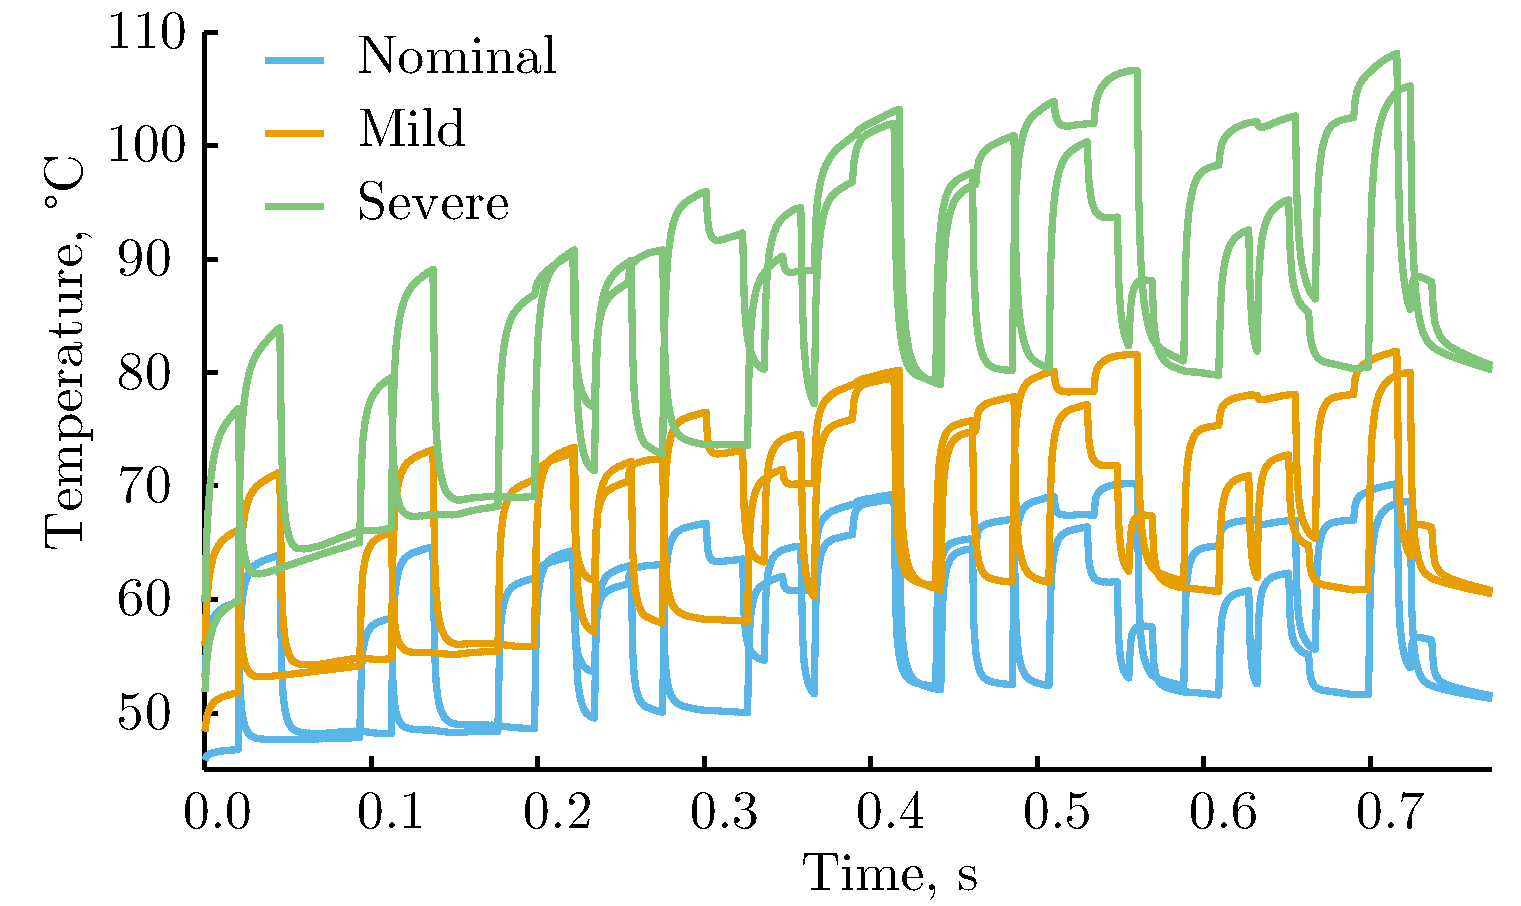
\includegraphics[width=1.0\linewidth]{include/assets/motivation-curve.pdf}
  \caption{Temperature fluctuation due to process variation.}
  \flabel{motivation-curve}
\end{figure}

\begin{figure}[br]
  \vspace{-1.5em}
  \centering
  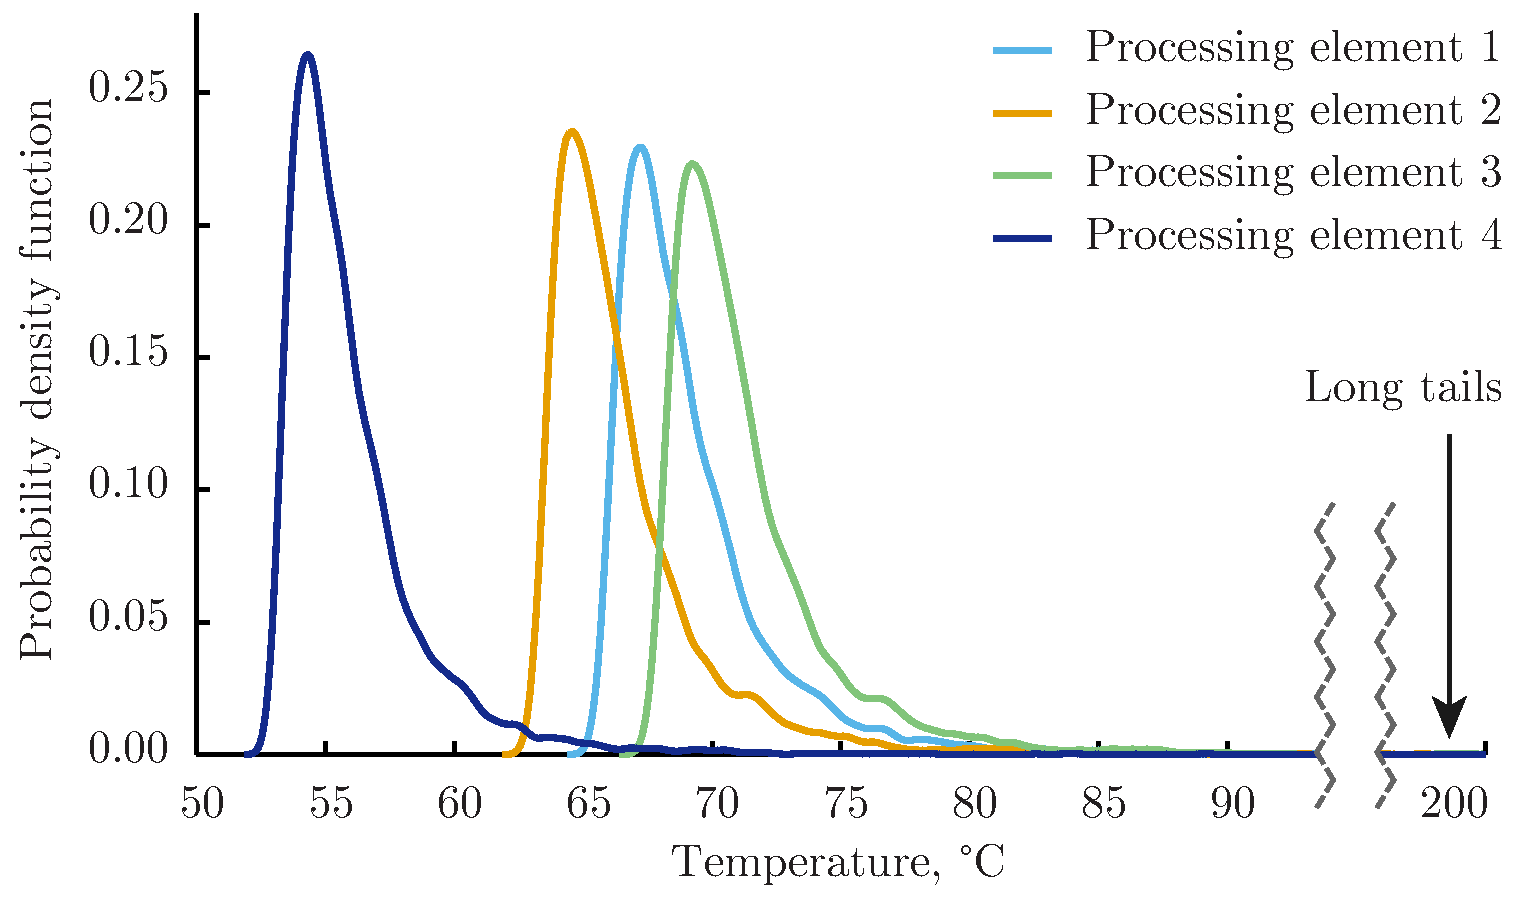
\includegraphics[width=1.0\linewidth]{include/assets/motivation-pdf.pdf}
  \caption{Probability density functions.}
  \flabel{motivation-pdf}
  \vspace{-1.0em}
\end{figure}

To overcome the limitations of deterministic PTA, a number of stochastic PTA techniques have been recently introduced. A solely power-targeted but temperature-aware solution is proposed in \cite{chandra2010}, which employs Monte Carlo (MC) simulations. A learning-based approach is presented in \cite{juan2011} to estimate the maximal temperature under the steady-state condition and variability of the leakage current. Leakage is also considered in \cite{juan2012}, where a statistical model of the steady-state temperature based on Gaussian distributions is derived. None of the aforementioned techniques attempts to perform the stochastic \emph{transient} PTA and to compute the evolving-in-time probability distribution of temperature. However, such transient curves are of practical importance. First of all, certain procedures cannot be undertaken without the knowledge of time-dependent temperature variations, \eg, the reliability optimization based on the thermal-cycling fatigue. Secondly, the constant steady-state temperature assumption, considered, \eg, in \cite{juan2011, juan2012}, can rarely be justified since power profiles are not invariant in reality. Thirdly, the frequently made assumption that power and/or temperature follow \apriori\ known probability distributions---for instance, Gaussian and log-normal distributions are popular choices, as in \cite{juan2012, srivastava2010}---is not realistic due to (a) the strict nonlinearities between the process parameters, power, and temperature; (b) the nonlinear interdependency of temperature and the leakage power \cite{liu2007}. To illustrate this, we simulated the previously mentioned example $10^4$ times with respect to the distribution of the parameters taken from literature (discussed in \sref{illustrative-example}), and performed kernel density estimation of probability density functions (\pdfs) of the temperature of the four processors at the middle of the time span shown in \fref{motivation-curve} (at time 0.39~s). The results are depicted in \fref{motivation-pdf}; and it can be seen that they are neither Gaussian nor log-normal. To conclude, the present stochastic PTA techniques for multiprocessor system design are restricted in use due to one or several of the following traits: based on MC simulations (potentially slow) \cite{chandra2010}, limited to power analysis \cite{chandra2010}, limited to the assumption of the constant steady-state temperature \cite{juan2011, juan2012}, exclusive focus on the maximal temperature \cite{juan2011}, \apriori\ chosen distributions of power and temperature \cite{juan2012, srivastava2010}. Consequently, there is a lack of flexible stochastic PTA techniques, which we aim to fulfill.

\begin{figure*}
  \vspace{-1.0em}
  \centering
  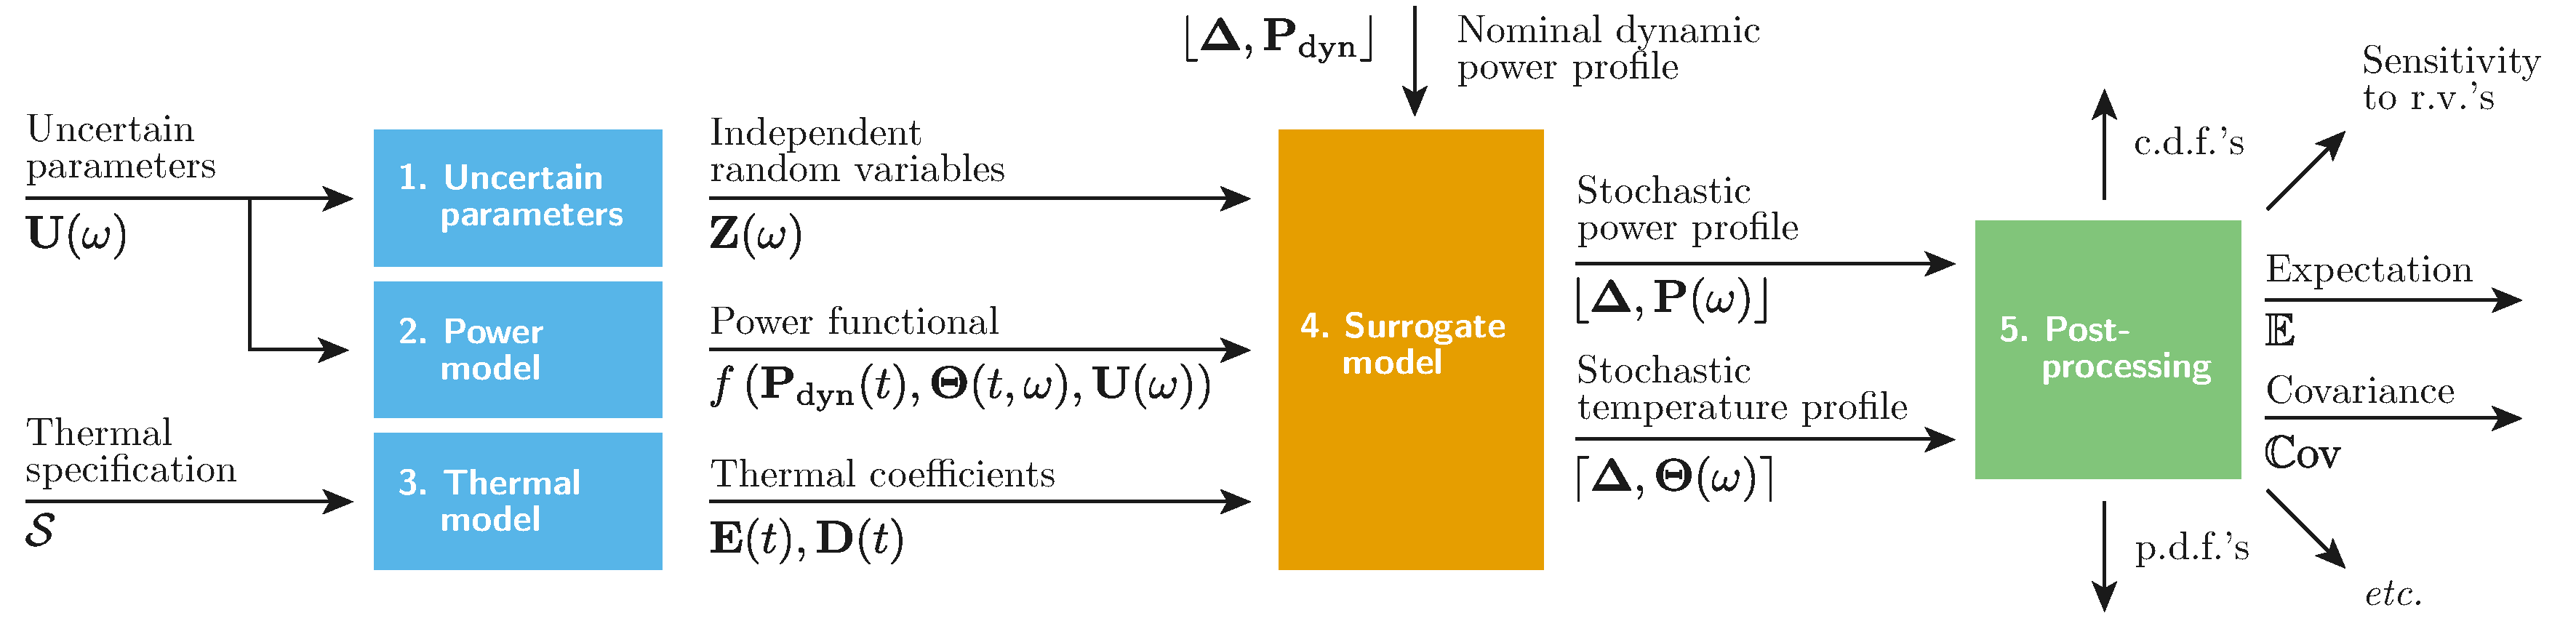
\includegraphics[width=1\textwidth]{include/assets/algorithm.pdf}
  \vspace{-1.0em}
  \caption{The structure of the proposed framework.}
  \flabel{algorithm}
  \vspace{-1.0em}
\end{figure*}

A straightforward approach to analyze a stochastic system is MC sampling coupled with a deterministic simulator. The major problem with MC sampling is the low rate of convergence, \eg, the mean value converges as $\mcsamples^{-\ifrac{1}{2}}$ where $\mcsamples$ is the number of samples \cite{xiu2010, maitre2010}. This means that, in order to get an additional decimal point of accuracy, one has to obtain hundred times more samples. Each such sample implies a complete realization of the whole system; therefore, MC-based methods are typically slow and often infeasible since the number of needed simulations can be extremely large \cite{diaz-emparanza2002}.

Attractive alternatives to MC sampling are spectral methods \cite{xiu2010, maitre2010} such as the generalized polynomial chaos (PC) \cite{xiu2002}, which is able to construct easy-to-analyze representations of system responses to stochastic inputs. PC is commonly accompanied by another spectral method known as the Karhunen-Lo\`{e}ve (KL) expansion \cite{ghanem1991}. KL is useful as a technique for reduction of the number of uncertain parameters and, hence, of the resulting computational costs. In \cite{shen2009}, PC based on Hermite polynomials is employed to estimate the full-chip leakage; the KL expansion is used in \cite{bhardwaj2006} to calculate the leakage current of electrical circuits; an analysis of the voltage response of power grids is carried out in \cite{ghanta2006}, where the PC and KL expansions are jointly utilized.

The contribution of this paper is in the following: we develop, for the first time, a framework for UQ of transient power and temperature variations of multiprocessor systems that depend on a number of uncertain parameters. The framework is flexible in modeling diverse probability distributions, specified by the user, of the parameters, and there are no assumptions on the distributions of the resulting power and temperature traces, as these distributions are unlikely to be known \apriori. Furthermore, our technique is capable of capturing arbitrary joint effects of the uncertain parameters on the system since the parameters are introduced into the model as a ``black box'', which is also defined by the user. The output of the framework is composed of the stochastic power and temperature profiles of the system given as polynomials of \rvs; the expressions are straightforward to be further analyzed. The framework is illustrated on one of the most important parameters affected by process variation: the subthreshold leakage current. Note, however, that our approach is not bounded to any particular source of variability and, apart from the process-related variations, can be applied to other uncertainties such as those due to environment, \ie, fluctuation of the supply voltage, ambient temperature, \etc

The reminder of the paper is organized as follows. In \sref{preliminaries}, we formulate the objective of our study. A brief overview of the proposed framework is given in \sref{overview}. In \sref{proposed-framework}, the framework is presented in details. A particular application is discussed in \sref{illustrative-example}, and the corresponding results are compared with MC simulations in \sref{experimental-results}. \sref{conclusion} concludes the paper. The work contains a set of supplementary materials with in-depth discussions on certain aspects of our approach.
